\scanpage{54}
\mspage{53}

D'abord, on va dégager les axiomes pour $\leq$

\uline{$\mathcal C$ 1} a) $\mathcal F\ne\varnothing$

\deleted{\uline{\unsure{C 2}}} b) Si $F\in\mathcal F_{\leq}$, et $(F_i)_{i\in I}$ est une famille d'objets de $\mathcal F$ avec $F_i\leq F$, alors $\underset{i}{\mathrm{Sup}}\,F_j$ existe. (Toute famille majorée de figures a une borne sup.)\figure{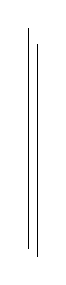
\begin{tikzpicture}\draw (0,0)--(0,2.8);\draw (.12,-.1)--(.12,2.6);\end{tikzpicture}}

\uline{Corollaire} $\mathcal F$ a un plus petit élé\deleted{\unsure{ment|mt}} (savoir, le $\mathrm{Sup}$ de la famille vide d'objets)

\uline{NB} En présence de \deleted{\unsure{C2}} \uline{C 1 b)}, la validité de a) \uline{équivaut} à celle du corollaire.

Le plus petit \unsure{élémt|élément} est appelé \uline{figure vide}, notée $\varnothing_{\mathcal F}$ ou simplement $\varnothing$, par abus de langage, et si confusion n'est à craindre

\figure{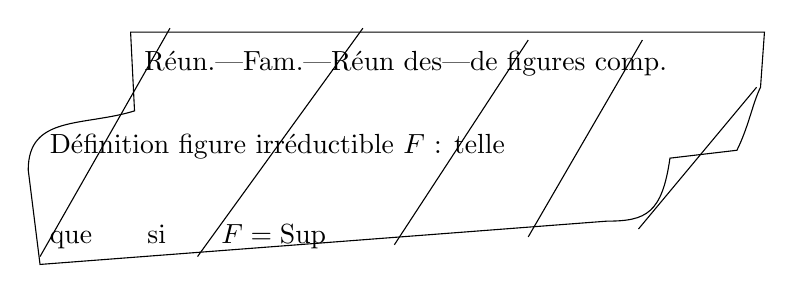
\begin{tikzpicture}[x=1cm,y=1cm]
\node[anchor=west] at (1.2,2.2) {\deleted{\unsure{Réun.|Fam.|Réun} \unsure{des|de} figures comp.}};
\node[anchor=west] at (0,1.15) {\deleted{\uline{Définition} \uline{figure} \uline{irréductible $F$ : telle}}};
\node[anchor=west] at (0,0) {\deleted{que\qquad si\qquad $F=\mathrm{Sup}$}};
\draw (1.15,2.6)--(9.2,2.6)--(9.15,1.9) .. controls (9.05,1.7) and (9.0,1.4) .. (8.85,1.1) -- (8.0,1.0) .. controls (7.9,.3) and (7.7,.2) .. (7.2,.2) -- (0,-.35)--(-.15,.85) .. controls (-.15,1.55) and (.55,1.4) .. (1.2,1.6)--cycle;
\draw (0,-.25)--(1.65,2.65) (2.0,-.25)--(4.1,2.65) (4.5,-.1)--(6.2,2.5) (6.2,0)--(7.65,2.5) (7.6,.1)--(9.1,1.9);
\end{tikzpicture}}

Figures \uline{compatibles}, ens de figures \deleted{\unsure{compatibles}} compatibles : \deleted{\unsure{un qui|qui}} \inserted{dans leur ens.} (ou \uline{configuration}) : qui est majoré pour $\leq$. \margin{P} Figure engendrée, ou \uline{réunion} ($F\vee G$, $\bigvee_i f_i$, $\mathrm{Sup}\,F_i$, parfois noté $F\cup G$ \unsure{ou|--} $\deleted{F}\bigcup_iF_i$ cf plus bas).

\uline{Déf} \uline{Figure irréductible} $F$ : telle que $\displaystyle F=\underset{i\in I}{\mathrm{Sup}}\,F_i\ \overset{-}{\Longrightarrow}\ \exists i\in I,\ F_i=F$.

\deleted{\uline{C 2}} Les figures irréductibles sont appelées des \uline{multistrates}. \inserted{L'ens des multistrates noté $ M$} Les figures irréductibles
